\documentclass[aps,pra,a4paper,twocolumn,10pt,superscriptaddress,longbibliography]{revtex4-1}

\usepackage[utf8]{inputenc}
\usepackage[english]{babel}
\usepackage[T1]{fontenc}
%\usepackage[sc,osf]{mathpazo}
\usepackage{times}
%\usepackage{pxfonts}

\usepackage{amsmath, amsthm, amssymb}
\usepackage{graphicx}
\usepackage{dcolumn}
\usepackage{dsfont}
\usepackage{bm}
\usepackage{color}
\usepackage[usenames,dvipsnames]{xcolor}
\usepackage{booktabs}
\usepackage{multirow}

\usepackage{changes}
\usepackage{verbatim}

%geometry for using a4paper
\usepackage{geometry}
\geometry{tmargin=2.5cm,bmargin=2.5cm,lmargin=2cm,rmargin=2cm}

%bibliography
%\usepackage[sort&compress]{natbib}

%figures
\DeclareGraphicsExtensions{.png,.pdf,.eps}
\graphicspath{ {./figs/} }
\renewcommand{\figurename}{Fig.}
%make less space below captions
\setlength{\belowcaptionskip}{-10pt}


%tables
\renewcommand\arraystretch{1}

%hyperref
\definecolor{myurlcolor}{rgb}{0,0,0.7}
\definecolor{myrefcolor}{rgb}{0.8,0,0}
\usepackage[unicode=true,pdfusetitle, bookmarks=false,bookmarksnumbered=false, bookmarksopen=false, breaklinks=false,pdfborder={0 0 0},backref=false, colorlinks=true, linkcolor=myrefcolor,citecolor=myurlcolor,urlcolor=myurlcolor]{hyperref}



%%%%%%%%%%%%%%%%%%%%%%%%%%%%%%%%%%%%%%%%%%%%%%%%%%%%%%%%%%%%%%%%%%%%
% MACROS
%%%%%%%%%%%%%%%%%%%%%%%%%%%%%%%%%%%%%%%%%%%%%%%%%%%%%%%%%%%%%%%%%%%%


% global
%%%%%%%%%%%%%%%%%%%%%%%%%%%%%%%%%%%%%%%%%%%%%%%%%%%%%%%%%%%%%%%%%%%%

% referencing
\newcommand{\eref}[1]{(\ref{#1})}
\newcommand{\eqnref}[1]{Eq.~(\ref{#1})}
\newcommand{\eqnsref}[2]{Eqs.~(\ref{#1}-\ref{#2})}
\newcommand{\figref}[1]{Fig.~\ref{#1}}
\newcommand{\tabref}[1]{Table~\ref{#1}}
\newcommand{\secref}[1]{Sec.~\ref{#1}}
\newcommand{\appref}[1]{App.~\ref{#1}}
\newcommand{\chapref}[1]{Chap.~\ref{#1}}
\newcommand{\citeref}[1]{Ref.~\cite{#1}}
\newcommand{\citerefs}[1]{Refs.~\cite{#1}}

% environments
% \theoremstyle{definition}
% \newtheorem{definition}{Definition}%[section]
% %
% \theoremstyle{plain}
% \newtheorem{lem}[definition]{Lemma}
% \newtheorem{fact}[definition]{Fact}
% \newtheorem{thm}[definition]{Theorem}
% \newtheorem{prop}[definition]{Proposition}
% \newtheorem{conj}[definition]{Conjecture}
% %
% %\newtheorem{lemma}{Lemma}[section]
% %\newtheorem{corollary}{Corollary}[section]
% %\newtheorem{protocol}{Protocol}[section]
% %\newtheorem{theorem}{Theorem}
% %\newtheorem{proposition}{Proposition}[section]
% %\newtheorem{definition}{Definition}[section]
% %\newtheorem{conjecture}{Conjecture}[section]
% %\newtheorem{fact}{Fact}[section]
% %\newtheorem{proof}{Proof}[section]
% %\newtheorem{remark}{Remark}[section]
% %
% \theoremstyle{remark}
% \newtheorem*{remark}{Remark}
% %

% real and imaginary part
\renewcommand\Re{\operatorname{Re}}
\renewcommand\Im{\operatorname{Im}}

% Dirac notation
\def \diracspacing {0.7pt}
\newcommand{\bra}[1]{\langle #1 \hspace{\diracspacing} |} % bra
\newcommand{\ket}[1]{| \hspace{\diracspacing} #1 \rangle} % ket
\newcommand{\braket}[2]{\langle #1 \hspace{\diracspacing} | \hspace{\diracspacing} #2 \rangle} % braket with different vectors
\newcommand{\braketq}[1]{\braket{#1}{#1}} % braket with the same vector
\newcommand{\ketbra}[2]{| \hspace{\diracspacing} #1 \rangle \langle #2 \hspace{\diracspacing} |} % ketbra with different vectors
\newcommand{\ketbras}[3]{| \hspace{\diracspacing} #1 \rangle_{#3} \langle #2 \hspace{\diracspacing} |} % ketbra with different vectors and a subscript
\newcommand{\ketbraq}[1]{\ketbra{#1}{#1}} % ketbra with the same vector
\newcommand{\bramatket}[3]{\langle #1 \hspace{\diracspacing} | #2 | \hspace{\diracspacing} #3 \rangle} % bra-matrix-ket with different vectors
\newcommand{\bramatketq}[2]{\bramatket{#1}{#2}{#1}} % bra-matrix-ket with the same vector

% text styles
\newcommand{\mrm}[1]{\mathrm{#1}}
\newcommand{\trm}[1]{\textrm{#1}}
\renewcommand{\t}[1]{\text{#1}}

% miscellaneous
\newcommand{\tran}[0]{^\textnormal{\tiny{T}}}
%\newcommand{\norm}[2][]{#1| \! #1| #2 #1| \! #1|}
\newcommand{\norm}[2][]{#1\left| \! #1\left| #2 #1\right| \! #1\right|}
\newcommand{\ave}[2][]{#1\langle #2 #1\rangle}
\newcommand{\abs}[2][]{#1| #2 #1|}
\newcommand{\I}{\mathbb{I}}
\newcommand{\cQ}{\mathcal{Q}}
\newcommand{\cL}{\mathcal{L}}
\newcommand{\cNL}{\mathcal{N\!L}}
\newcommand{\cH}{\mathcal{H}}
\newcommand{\cB}{\mathcal{B}}
\newcommand{\cC}{\mathcal{C}}
\newcommand{\cS}{\mathcal{S}}
\newcommand{\cNC}{\mathcal{NC}}
\newcommand{\bC}{\mathbb{C}}
\newcommand{\tp}{\tilde{p}}
\newcommand{\tA}{\tilde{A}}
\newcommand{\tB}{\tilde{B}}
\newcommand{\ha}{\hat{a}}
\newcommand{\hb}{\hat{b}}
\newcommand{\ba}{\bar{a}}
\newcommand{\bb}{\bar{b}}

\newcommand{\be}{\bar{e}}
\newcommand{\bE}{\bar{E}}
\newcommand{\la}{\langle}
\newcommand{\ra}{\rangle}
%
%\DeclareMathOperator{\tr}{tr}
\DeclareMathOperator{\Ext}{Ext}


\newcommand{\tr}[1]{\mrm{Tr}\!\left\{{#1}\right\}}

\newcommand{\mat}[1]{\bm{\mathit{#1}}}

% local to this manuscript
%%%%%%%%%%%%%%%%%%%%%%%%%%%%%%%%%%%%%%%%%%%%%%%%%%%%%%%%%%%%%%%%%%%%
\newcommand{\CHSH}{\text{CHSH}}
\newcommand{\ro}{r_{\text{1-way}}}
\newcommand{\rt}{r_{\text{2-way}}}
\newcommand{\rDW}{r_{\text{DW}}}
\newcommand{\rUB}[1]{r^\uparrow_{\text{#1}}}
\newcommand{\neta}{\bar{\eta}}
\newcommand{\nq}{\bar{q}}

%notations for correlations
\newcommand{\sub}[1]{\mrm{#1}}
\newcommand{\p}[1]{p_\sub{#1}}

\newcommand{\pAB}{\p{AB}}
\newcommand{\pABobs}{\p{AB}^\trm{obs}} %observed
\newcommand{\pobs}{p^\trm{obs}} %observed

\newcommand{\pABE}{\p{ABE}}
\newcommand{\pA}{\p{A}}
\newcommand{\pB}{\p{B}}
\newcommand{\pE}{\p{E}}


\newcommand{\rhoAB}{\rho_\sub{AB}}
\newcommand{\rhoABE}{\rho_\sub{ABE}}
\newcommand{\QAB}{Q_\sub{AB}}

%numbers of measuement settings
\newcommand{\mA}{m_\sub{A}}
\newcommand{\mB}{m_\sub{B}}
%numbers of measuement outcomes
\newcommand{\nA}{n_\sub{A}}
\newcommand{\nB}{n_\sub{B}}

%key settings
\newcommand{\xk}{x^*}
\newcommand{\yk}{y^*}

%probabilities vectors
\newcommand{\pvec}{\textbf{p}}
\newcommand{\qvec}{\textbf{q}}

\newcommand{\ox}{\textrm{O}}
\newcommand{\vegf}{\textrm{V}}
\newcommand{\sig}{\textrm{S}}

%%%%%%%%%%%%%%%%%%%%%%%%%%%%%%%%%%%%%%%%%%%%%%%%%%%%%%%%%%%%%%%%%%%%

% comments
\newcommand{\jk}[1]{{\color{blue} #1}}
\newcommand{\jkC}[1]{\jk{[JK:~#1]}}
\newcommand{\kl}[1]{{\textcolor{cyan}{#1}}}
\newcommand{\klC}[1]{\kl{[Karol:~#1]}}
\newcommand{\mateC}[1]{\textcolor{magenta}{[mate: #1]}}
\newcommand{\mate}[1]{\textcolor{magenta}{#1}}
\newcommand{\toni}[1]{\textcolor{red}{#1}}








\begin{document}

\title{A lattice model of vascular network formation}


\author{(alphabetical) K\L, AMN, TS, PS}

\begin{abstract}
We consider a minimalistic model of blood vessel formation and remodelling starting from the capillary plexus. The vascular network grows in a response to the vascular endothelial growth factor (VEGF) released by the oxygen-deprived cells. The network is further remodeled in response to the shear stress at the vessel walls. Two additional phenomena are taken into account: the first is the conduction of metabolic stimulus for diameter increase along the vessel walls, the second is the driving role of the blood flow in the sprout formation and elongation. Together, these mechanisms are able to create and sustain long loops in the network, formed by arterioles, connecting capillaries and venules. These loops are  capable of efficiently oxygenating even the remotest areas of the network, regardless of the geometry. We quantify the effects of VEGF-driven growth and shear-stress remodeling and compare the results with the real cases of neovascularization.
\end{abstract}

\maketitle





%%%%%%%%%%%%%%%%%%%%%%%%%%%%%%%%%%%%%%%%%%%%%%%%%%%%%%%%%%%%%%%%%%%%%%%%%%%%%%%%%%%%%%%%%%%%%
%%%%%%%%%%%%%%%%%%%%%%%%%%%%%%%%%%%%%%%%%%%%%%%%%%%%%%%%%%%%%%%%%%%%%%%%%%%%%%%%%%%%%%%%%%%%%
\section{Introduction}
\label{sec:intro}
%%%%%%%%%%%%%%%%%%%%%%%%%%%%%%%%%%%%%%%%%%%%%%%%%%%%%%%%%%%%%%%%%%%%%%%%%%%%%%%%%%%%%%%%%%%%%
%%%%%%%%%%%%%%%%%%%%%%%%%%%%%%%%%%%%%%%%%%%%%%%%%%%%%%%%%%%%%%%%%%%%%%%%%%%%%%%%%%%%%%%%%%%%%
%
\emph{Motivation.} Historical background, existing models. Goal of this model: to have complex behaviour (network resembling vasculature) emerge from simple rules.

%
\emph{Quality of the model}. Judged by the amount of oxygenation in the simulated area (alternatively, amount of VEGF).

%
\emph{Basic setup.} Evolution of a 2D network. Starts from a capillary plexus with the edges of the network corresponding to individual blood vessels (modelled as cylindrical tubes), nodes corresponding to connections between them. Network evolves by changing the diameters of the vessels, which happens in response to several factors (evolution mechanisms).

%
\emph{Evolution mechanisms.} Shear stress at the vessel walls dependent on the flow parameters induces diameter growth. Concentration of the vascular endothelial growth factor (VEGF) and oxygen is tracked at each node, the former diffusing due to the lack of the latter, promoting vessel growth in the direction of the hypoxic region. Metabolic signal is conducted upstream and downstream along the vessels, inducing diameter growth in vessels responsible for the delivery of oxygen into the hypoxic regions.

%
%%%%%%%%%%%%%%%%%%%%%%%%%%%%%%%%%%%%%%%%%%%%%%%%%%%%%%%%%%%%%%%%%%%%%%%%%%%%%%%%%%%%%%%%%%%%%
%%%%%%%%%%%%%%%%%%%%%%%%%%%%%%%%%%%%%%%%%%%%%%%%%%%%%%%%%%%%%%%%%%%%%%%%%%%%%%%%%%%%%%%%%%%%%
\section{Lattice model of vascular network formation}
\label{sec:model}
%%%%%%%%%%%%%%%%%%%%%%%%%%%%%%%%%%%%%%%%%%%%%%%%%%%%%%%%%%%%%%%%%%%%%%%%%%%%%%%%%%%%%%%%%%%%%
%%%%%%%%%%%%%%%%%%%%%%%%%%%%%%%%%%%%%%%%%%%%%%%%%%%%%%%%%%%%%%%%%%%%%%%%%%%%%%%%%%%%%%%%%%%%%
%
\emph{Network setup.} Network constructed by randomly selecting points on a square area and connecting them by Delaunay triangulation. Each edge (vessel) characterized by its length (unchanging in the simulation), diameter (evolved via the evolution mechanisms; initially having a Gaussian distribution across the network). Furthermore, each vessel is classified as either a \emph{capillary}, a \emph{venule} or an \emph{arteriole}. A capillary is promoted to a venule (arteriole) upon exceeding a set diameter threshold and if it's already connected to an existing venule (arteriole). A set of nodes $\mathcal{I}$ is chosen to be the \emph{input} nodes, through which a constant inflow of blood $Q$ is introduced into the system; conversly, $\mathcal{O}$ is the set of \emph{output} nodes through which a constant outflow of blood $Q$ is taken out of the system. Each node $i$ is characterized by the pressure $p_i$ exerted at its location by the fluid, local concentration of oxygen $c_{\ox,i}$, local concentration of VEGF $c_{\vegf,i}$ and the local value of the metabolic signal $c_\sig$.
\begin{figure}[h!]
\centering
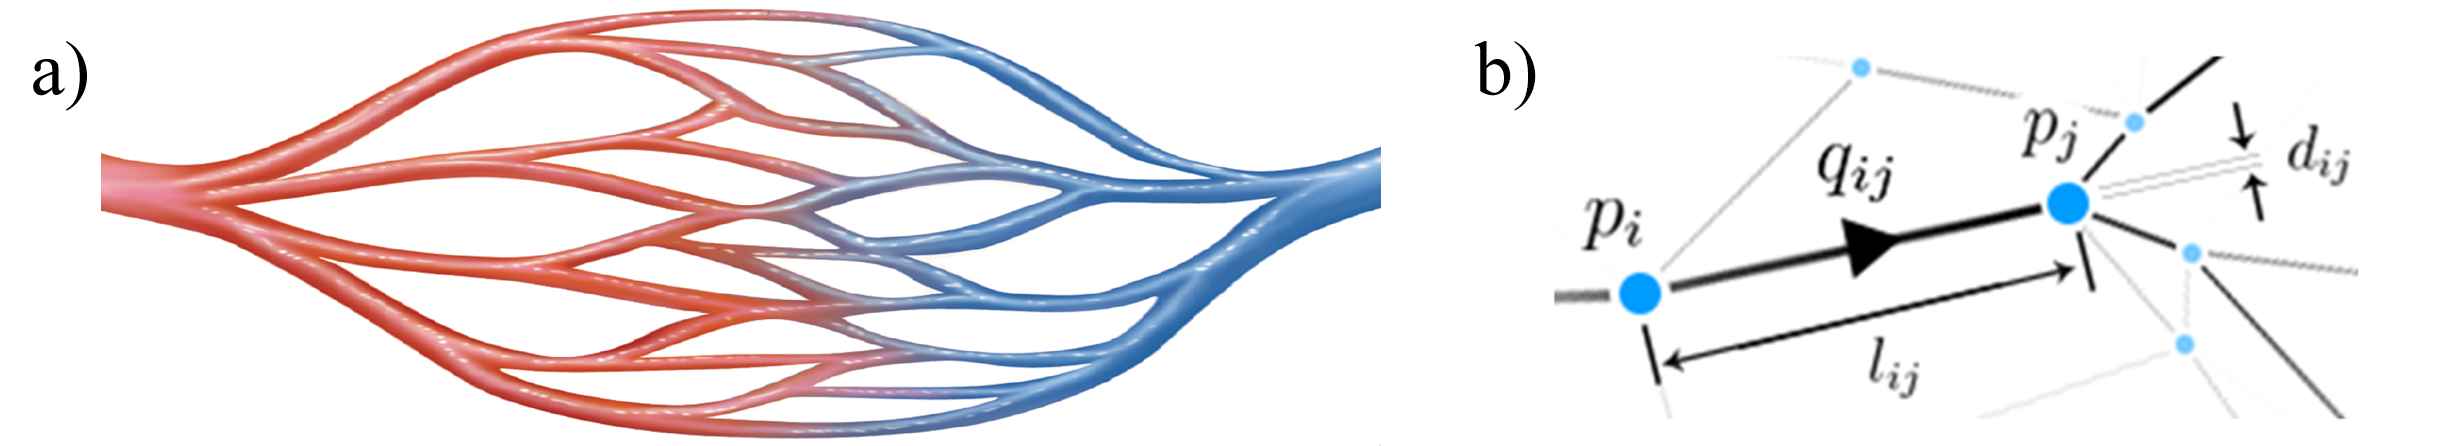
\includegraphics[width=\columnwidth]{fig1_vessel-division_schematic.png}
\caption{a) Division into capillaries, venules and arterioles. b) Schematic representation of the network parameters.}
\label{fig:division}
\end{figure}
%%%%%%%%%%%%%%%%%%%%%%%%%%%%%%%%%%%%%%%%%%%%%%%%%%%%%%%%%%%%%%%%%%%%%%%%%%%%%%%%%%%%%%%%%%%%%
%%%%%%%%%%%%%%%%%%%%%%%%%%%%%%%%%%%%%%%%%%%%%%%%%%%%%%%%%%%%%%%%%%%%%%%%%%%%%%%%%%%%%%%%%%%%%
%

\emph{Quasistatic evolution mechanisms.} 
The network is evolved slowly, i.e., in each iteration the system is allowed to relax to an equilibrium state. In effect, all the equations are solved for the steady-state case with time derivatives vanishing.
%%%%%%%%%%%%%%%%%%%%%%%%%%%%%%%%%%%%%%%%%%%%%%%%%%%%%%%%%%%%%%%%%%%%%%%%%%%%%%%%%%%%%%%%%%%%%
%%%%%%%%%%%%%%%%%%%%%%%%%%%%%%%%%%%%%%%%%%%%%%%%%%%%%%%%%%%%%%%%%%%%%%%%%%%%%%%%%%%%%%%%%%%%%
%
\paragraph{Pressure, flow, shear stress.}
In each iteration first the pressure and flow values are determined, according to the current parameters of the network. Specifically, fluid flow in each elementary vessel connecting nodes $i$ and $j$ satisfies the Hagen-Poiseuille equation
\begin{equation}
\label{eq:hagen-poiseuillie}
q_{ij} = \lambda_{ij} (p_i - p_j)
\end{equation}
where
\begin{equation}
\lambda_{ij} := \frac{\pi d_{ij}^4}{128 \mu_{ij} l_{ij}}
\end{equation}
Input boundary conditions are set to constant input pressure
\begin{equation}
p_{i \in \mathcal{I}} =: p_\t{in} = \mathrm{const}
\end{equation}
and constant inflow
\begin{equation}
\begin{aligned}
Q &= \sum_{i \in \mathcal{I}} \sum_{j} q_{ij} = \sum_{i \in \mathcal{I}} \sum_{j} \lambda_{ij} (p_\t{in} - p_j) \\ &= p_\t{in} \left( \sum_{i \in \mathcal{I}} \sum_{j} \lambda_{ij} \right) - \sum_{i \in \mathcal{I}} \sum_{j} \lambda_{ij} p_j.
\end{aligned}
\end{equation}
Output boundary condition is set to
\begin{equation}
p_{i \in \mathcal{O}} = 0.
\end{equation}
The continuity condition requires
\begin{equation}
\sum_{j} q_{ij} = p_i \sum_{j} \lambda_{ij} - \sum_{j} \lambda_{ij} p_j = 0 \quad \forall i \not\in \mathcal{I}, \mathcal{O}.
\end{equation}
Therefore, the pressure vector $\mathbf{p}$ has to satisfy the following matrix equation
\begin{equation}
\mat{\Lambda} \cdot \mathbf{p} = \mathbf{q}
\end{equation}
where
\begin{alignat}{3}
& \forall i \not\in \mathcal{I}, \mathcal{O} \; && \left[\mat{\Lambda}\right]_{i \neq j} = -\lambda_{ij}, \; & &  \left[\mat{\Lambda}\right]_{i i} = \sum_{j} \lambda_{ij}\\
& \forall i \in \mathcal{I} \; && \left[\mat{\Lambda}\right]_{i \neq j} = \sum_{k \in \mathcal{I}} \lambda_{kj}, \; & & \left[\mat{\Lambda}\right]_{i i} =  \sum_{k \in \mathcal{I}} \sum_{j} \lambda_{kj}\\
& \forall i \in \mathcal{O} \; && \left[\mat{\Lambda}\right]_{i \neq j} = 0, \; & & \left[\mat{\Lambda}\right]_{i i} = 1
\end{alignat}
and 
\begin{equation}
\left[\mathbf{q}\right]_{i \in \mathcal{I}} = Q, \quad \left[\mathbf{q}\right]_{i \not\in \mathcal{I}} = 0. 
\end{equation}

Flow of blood induces shear stress at the vessel walls given by 
\begin{equation}
\label{eq:shear-stress}
\tau_{ij} = 2 \mu_{ij} \frac{\mathrm{d}v_{ij}}{\mathrm{d}r} \Big |_{r = d_{ij} / 2}
\end{equation}
where $v_{ij}(r)$ is the velocity of the fluid at radius $r$ from the cylinder's axis, assumed to have a parabolic profile
\begin{equation}
\label{eq:parabolic-vel}
v_{ij}(r) = \frac{G}{4 \mu_{ij}} \left[ \left(\frac{d_{ij}}{2}\right)^2 - r^2 \right ]
\end{equation}
with $G$ a constant to be determined. Integrating the velocity over the vessel's cross-section and comparing with \eqref{eq:hagen-poiseuillie}, as well as combining \eqref{eq:shear-stress} with \eqref{eq:parabolic-vel}, allows one to find $G$ and obtain
\begin{equation}
\tau_{ij} = \frac{d_{ij} (p_i - p_j)}{2 l_{ij}}.
\end{equation}
In every iteration, after calculating the shear stress in each vessel, the diameters $d_{ij}$ are updated according to a chosen rule. Specifically...
%%%%%%%%%%%%%%%%%%%%%%%%%%%%%%%%%%%%%%%%%%%%%%%%%%%%%%%%%%%%%%%%%%%%%%%%%%%%%%%%%%%%%%%%%%%%%
%%%%%%%%%%%%%%%%%%%%%%%%%%%%%%%%%%%%%%%%%%%%%%%%%%%%%%%%%%%%%%%%%%%%%%%%%%%%%%%%%%%%%%%%%%%%%
%

\paragraph{Oxygen in the arterioles.}
Arterioles are supposed to introduce oxygen into the system, thus a boundary condition
\begin{equation}
c_{\ox, i\in\mathcal{I}} = 1
\end{equation}
is assumed and used to solve a convection-reaction equation in the arterioles, given by (in the continuous case)
\begin{equation}
q\, \nabla c_{\ox} = - k_a c_{\ox}
\end{equation}
where the LSH describes the convection of oxygen with the blood flow and the RHS models oxygen decay/concentration drop along the arterioles with rate $k_a$. This has the effect of the oxygen being well distributed along the vessels with high flow and less so along flow-deficient vessels.
%

\paragraph{Oxygen in the capillary bed.}
Oxygen concentration in the arterioles calculated in the previuos step, along with setting $c_\ox = 0$ in the venules, are taken as boundary conditions to the diffusion-reaction equation for $c_{\ox}$ computed in the rest of the lattice,
\begin{equation}
D_{\ox} \, \Delta c_{\ox} = k_{\ox} c_{\ox},
\end{equation}
where $D_{\ox}$ and $k_{\ox}$ are the oxygen diffusion constant and oxygen reaction constant, respectively. 
%

\paragraph{VEGF.}
VEGF is produced in hypoxic regions and diffuses throughout the network according to a diffusion-reaction equation
\begin{equation}
D_{\vegf} \, \Delta c_{\vegf} = -R(c_\ox),
\end{equation}
where $D_\vegf$ is the VEGF diffusion constant and $R$ should be a decreasing function of $c_\ox$. Then, vessel growth is promoted proportionally to the VEGF gradient in along it. Specifically...
\begin{figure}[h!]
\centering
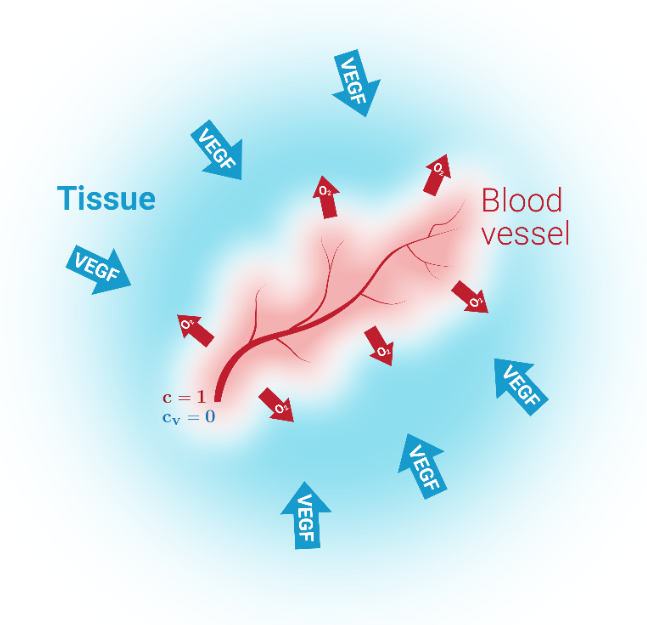
\includegraphics[width=\columnwidth]{schematic-vegf.png}
\caption{VEGF is produced in hypoxic regions and diffuses throughout the network. Vessel growth is promoted proportionally to the VEGF gradient.}
\label{fig:vegf-schematic}
\end{figure}

%
\paragraph{Metabolic signal.}
Emmited upwards and downwards from the nodes, signals to vessels further down/up the stream that a widening is needed for the delivery of oxygen. Signal concentration is governed by a diffusion-reaction equation
\begin{equation}
v_\sig \, \nabla c_\sig = R_\sig - k_\sig c_\sig,
\end{equation}
where in the reaction term on the RHS, $R_\sig$ is the production rate (VEGF-dependent?) and $k_\sig$ is the decay rate. Diameters are changed according to...
\begin{figure}[h!]
\centering
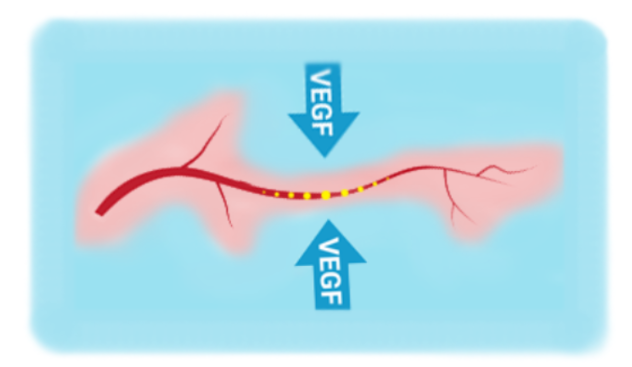
\includegraphics[width=\columnwidth]{signal-schematic.png}
\caption{Metabolic signal.}
\label{fig:signal-schematic}
\end{figure}

%
\emph{Algorithm summary.} 
See analogous summary in Pries.
%
%%%%%%%%%%%%%%%%%%%%%%%%%%%%%%%%%%%%%%%%%%%%%%%%%%%%%%%%%%%%%%%%%%%%%%%%%%%%%%%%%%%%%%%%%%%%%
%%%%%%%%%%%%%%%%%%%%%%%%%%%%%%%%%%%%%%%%%%%%%%%%%%%%%%%%%%%%%%%%%%%%%%%%%%%%%%%%%%%%%%%%%%%%%
%
\section{Results and discussion}
\label{sec:results}
%%%%%%%%%%%%%%%%%%%%%%%%%%%%%%%%%%%%%%%%%%%%%%%%%%%%%%%%%%%%%%%%%%%%%%%%%%%%%%%%%%%%%%%%%%%%%
%%%%%%%%%%%%%%%%%%%%%%%%%%%%%%%%%%%%%%%%%%%%%%%%%%%%%%%%%%%%%%%%%%%%%%%%%%%%%%%%%%%%%%%%%%%%%
%
\subsection{Beautiful pictures, amazing simulation!}
%
\subsection{Effect of the evolution mechanisms}
\emph{Shear stress.} Appearance of breakthroughs/short circuits. Shear on its own is not enough.

\emph{VEGF.} Also not enough on its own.

\emph{Metabolic signal.} Ladder sustained.
%
%%%%%%%%%%%%%%%%%%%%%%%%%%%%%%%%%%%%%%%%%%%%%%%%%%%%%%%%%%%%%%%%%%%%%%%%%%%%%%%%%%%%%%%%%%%%%
%%%%%%%%%%%%%%%%%%%%%%%%%%%%%%%%%%%%%%%%%%%%%%%%%%%%%%%%%%%%%%%%%%%%%%%%%%%%%%%%%%%%%%%%%%%%%
\section{Analysis}
\label{sec:analysis}
%%%%%%%%%%%%%%%%%%%%%%%%%%%%%%%%%%%%%%%%%%%%%%%%%%%%%%%%%%%%%%%%%%%%%%%%%%%%%%%%%%%%%%%%%%%%%
%%%%%%%%%%%%%%%%%%%%%%%%%%%%%%%%%%%%%%%%%%%%%%%%%%%%%%%%%%%%%%%%%%%%%%%%%%%%%%%%%%%%%%%%%%%%%
%
Strahler, angles, oxygenation. Comparison with real-life pictures.
%
%%%%%%%%%%%%%%%%%%%%%%%%%%%%%%%%%%%%%%%%%%%%%%%%%%%%%%%%%%%%%%%%%%%%%%%%%%%%%%%%%%%%%%%%%%%%%
%%%%%%%%%%%%%%%%%%%%%%%%%%%%%%%%%%%%%%%%%%%%%%%%%%%%%%%%%%%%%%%%%%%%%%%%%%%%%%%%%%%%%%%%%%%%%
\section{Summary}
\label{sec:sumarry}
%%%%%%%%%%%%%%%%%%%%%%%%%%%%%%%%%%%%%%%%%%%%%%%%%%%%%%%%%%%%%%%%%%%%%%%%%%%%%%%%%%%%%%%%%%%%%
%%%%%%%%%%%%%%%%%%%%%%%%%%%%%%%%%%%%%%%%%%%%%%%%%%%%%%%%%%%%%%%%%%%%%%%%%%%%%%%%%%%%%%%%%%%%%
%

\section*{TO ADD:}
%%%%%%%%%%%%%%%%%%%%%%%%%%%%%%%%%%%%%%%%%%%%%%%%%%%%%%%%%%%%%%%%%%%%%%%%%%%%%%%%%%%%%%%%%%%%%
%%%%%%%%%%%%%%%%%%%%%%%%%%%%%%%%%%%%%%%%%%%%%%%%%%%%%%%%%%%%%%%%%%%%%%%%%%%%%%%%%%%%%%%%%%%%%
%
\begin{itemize}
\item Geometry?
\item Describe constants (Damkohler number etc.)
\end{itemize}




%%%%%%%%%%%%%%%%%%%%%%%%%%%%%%%%%%%%%%%%%%%%%%%%%%%%%%%%%%%%%%%%%%%%%
\section*{Acknowledgements}
%
We thank Annemiek Cornelissen and Stéphane Douady for fruitful discussions. This work was supported by...


%\bibliographystyle{apsrev4-1}
\bibliography{vascular-network}





\end{document}